\section{Use Case and Evaluation}%
\label{sec:use-case-and-evaluation}


The research on KIF was in part motivated by the development of a chat-bot for the domain of chemistry.
%%
Depending on the user's question, the bot would retrieve statements about chemical compounds from various sources and present them as ``known facts''.
%%
There were three main requirements: (i)~the retrieved statements should be comparable, i.e., they should use the same vocabulary when talking about the same things; (ii)~their origin should be traceable, i.e., statements should come with provenance information; and (iii)~it should be easy to add new sources to the system.


Figure~\ref{fig:use-case} shows the instantiation of KIF used in the chat-bot application.
%%
A mixer store is used to combine three SPARQL stores: one pointing to a local installation of PubChem's RDF~\cite{Fu-G-2015} running on Virtuoso~\cite{Erling-O-2012}, one pointing to Wikidata's public SPARQL endpoint (WDQS), and one pointing to a local SPARQL endpoint built by Ontop over the SQL endpoint of IBM CIRCA\@.


\begin{figure}[b]
  \centering
  \begin{tikzpicture}[
    node distance=.5em,font=\rmfamily\footnotesize,
    cyl/.style={cylinder,aspect=.15,shape border rotate=90,inner sep=2pt}]
    \node[draw,minimum width=22em,minimum height=2em](mx){\strut Mixer};
    \begin{scope}[minimum width=7em, minimum height=2em,font=\scriptsize]
      \node[draw,below=of mx.south west,anchor=north west](S1){SPARQL Store};
      \node[draw,below=of mx.south,anchor=north](S2){SPARQL Store};
      \node[draw,below=of mx.south east,anchor=north east](S3){SPARQL Store};
    \end{scope}
    \begin{scope}[node distance=2em]
      \node[draw,minimum width=7em, minimum height=2em,below=of S3]
      (Ontop){\strut Ontop};
    \end{scope}
    \begin{scope}[node distance=1em,overlay,font=\scriptsize]
      \node[left=of S1,text width=3.75em,align=center](MS1){mapping\\(KIF)};
      \node[right=of Ontop,text width=3.75em,align=center]
      (MOntop){mapping\\(R2RML)};
      \draw[->](MS1) to (S1);
      \draw[->](MOntop) to (Ontop);
    \end{scope}
    \begin{scope}[font=\scriptsize,node distance=.5em]
      \node[draw,cyl,below=of Ontop,text width=3em,align=center]
      (CIRCA){IBM CIRCA};
      \node[draw,cyl,text width=3em,align=center]
      (Wikidata) at (S2|-CIRCA) {Wiki\-data};
      \node[draw,cyl,text width=3em,align=center]
      (PubChem) at (S1|-CIRCA) {Pub\-Chem};
    \end{scope}
    \draw(PubChem) to (S1);
    \draw(Wikidata) to (S2);
    \draw(CIRCA) to (Ontop);
    \draw(Ontop) to (S3);
    \coordinate(Y) at ($(Ontop)!.5!(S3)+(9,0)$);
    \coordinate(X) at ($(S1|-Y)+(-9,0)$);
    \draw[dashed](X) -- (Y);
    \begin{scope}
      \node[anchor=north west,yshift=-.25em] at (X){knowledge sources};
      \node[anchor=south east,yshift=.25em] at (Y){KIF};
    \end{scope}
  \end{tikzpicture}
  \caption{KIF instantiation integrating PubChem, Wikidata, and IBM CIRCA.}%
  \label{fig:use-case}
\end{figure}


%%% Local Variables:
%%% mode: latex
%%% TeX-engine: xetex
%%% TeX-master: "../main"
%%% eval: (visual-line-mode 1)
%%% End:



IBM CIRCA~\cite{IBM-CIRCA} is a relational database of chemical data extracted from patents and other sources.
%%
In the chat-bot application, we used Ontop to build a Wikidata-compatible SPARQL endpoint to access parts of its schema.
%%
Ontop~\cite{Xiao-G-2020} is an ontology-based data access tool.
%%
It uses R2RML~\cite{Cyganiak-R-2012} mappings to translate SPARQL queries to SQL at query time.
%%
The R2RML mappings tell Ontop how to map tables in the relational database into concepts and properties of the target ontology (in our case, Wikidata's).


\subsection{Evaluation}


For the evaluation, we used the setup shown in Figure~\ref{fig:use-case} without the IBM CIRCA part, i.e., essentially the setup shown in line~33 of Section~\ref{sub:the-mixer-store}.
%%
Our goal was to measure the overhead of KIF when evaluating simple application-level queries over the mixer.
%%
By overhead, we mean time spent in KIF (Python code) versus time spent in the SPARQL endpoints (outside the Python code).
%%
By simple application-level queries, we mean statement patterns meaningful to users.


For the experiment, we generated patterns of the forms
\[
  \text{\code/!$p$!(x,!$v_1$!).where(!$q$!(x,!$v_2$!))/}
  \quad\text{and}\quad
  \text{\code/!$p$!(!$v_1$!,x).where(!$q$!(x,!$v_2$!))/},
\]
where \code/x/ is a pattern variable, $p$ and $q$ are properties, $v_1$ is a value or variable, and $v_2$ is a value.
%%
Since we wanted matches in both Wikidata and PubChem, we restricted $p$ to the properties in PubChem whose domain or range is a chemical compound (e.g., mass (P2067), has part (P527), trading name (P6427), etc.) and $q$ to those which are compound identifiers (e.g., InChIKey (P235), canonical SMILES (P233), ChEBI ID (P683), etc.).


We evaluated each of the generated patterns over the mixer of Figure~\ref{fig:use-case} and collected those which (i) matched at least one statement in both Wikidata and PubChem, and (ii) took at least 0.75s to run in each of the endpoints.
%%
We then sorted the patterns by number of matches and selected the last~100 patterns.
%%
We ended up with patterns Q0--Q99, whose evaluation times are shown in Figure~\ref{fig:plot}.


\begin{figure}[ht]
  \centering
  \relax{\includegraphics[
    clip,
    trim=4.1em .5em 5.9em 2.2em,%lbrt
    width=.9\textwidth]{eval/plot.eps}}%
  \caption{%%
    KIF overhead.
    %%
    The x-axis shows the queries sorted by number of matches.
    %%
    The numbers above the red line indicate the number of matches for a particular query.
    %%
    The y-axis shows the time in seconds (in log scale).
    %%
    On average, 2.1\% of the time was spent in KIF, 12.4\% in Wikidata, and 85.5\% in PubChem.}%
  \label{fig:plot}
\end{figure}


For each pattern $Q_i$ in Figure~\ref{fig:plot}, the red line (Total) indicates the time taken to evaluate and consume all results of the call \code{match(!$Q_i$!)} over the mixer.
%%
The orange and green lines (Wikidata and PubChem) indicate the time taken to send the SPARQL queries to the endpoints and receive the results.
%%
The blue line (KIF) indicates the time spent in KIF where $\text{KIF}=\text{Total}-(\text{Wikidata}+\text{PubChem})$.


As expected, the bulk of the time (on average 97.9\%) was spent in the endpoints, in particular, PubChem.
%%
The overhead of KIF is negligible, especially when the number of matches is smaller than the page-size configured in KIF\@.
%%
In this experiment, we used a page of size~100, which is the default.
%%
This means that to consume a response with 1000 matches, KIF has to perform 10 requests.
%%
This explains the increase in the overhead of KIF after~Q70.
%%
Nevertheless, evaluation time is dominated by the SPARQL endpoints.


% LocalWords:  KIF PubChem's WDQS Ontop RML PubChem InChIKey ChEBI



%%% Local Variables:
%%% mode: latex
%%% TeX-engine: xetex
%%% TeX-master: "main"
%%% eval: (visual-line-mode 1)
%%% End:
